\documentclass[12pt]{report}
\usepackage[utf8]{inputenc}
\usepackage{tabularx}
\usepackage{float}
\usepackage{graphicx}
\usepackage{hyperref}
\hypersetup{
    colorlinks,
    citecolor=black,
    filecolor=black,
    linkcolor=black,
    urlcolor=black
}
\usepackage{makeidx}
\makeindex

\title{Semi Anonymous image-based message board \\ 
        \large Software Requirements Specification(SRS) Document}
\author{Group No. 24\\Sahil Gangurde (2019IMT-034)\\Anish Jaiswal (2019IMT-017)\\Shashi Kumar (2019IMT-090)}
\date{ABV - Indian Institute of Information Technology, Gwalior}

\begin{document}

\maketitle

\newpage
\tableofcontents
\newpage

\chapter{Introduction}
This section will give the scope\index{scope} and overall idea of the everything included in this SRS document. Also the purpose and list of abbreviations and definitions is also provided further.

\section{Purpose}
The purpose\index{purpose} of this document is to give the detailed requirement study for 'Semi-autonomous image based message board' website. It will illustrate the purpose and complete declaration for the development of system. It will also explain system constraints, interface and interactions with other external applications. This document is primarily intended to be proposed to a customer for its approval and a reference for developing the first version of the system for the development team.

\section{Scope}
This website is targeted to be made as a discussion forum where every discussion will start with a image posted by the user followed by users commenting and reacting to the image. Each user can also create different board(sub topics) where discussions about related images can happen. This website can be accessed by anyone having internet connection and a browser.

Registered users can create boards\index{boards}(subtopics), react to a post via upvoting or downvoting them and also can comment on the posts. This website also incorporated a anonymous user\index{anonymous user} feature where anonymous users can comment on the posts created by registered users. There is no admin panel as such for this website as the purpose of this website is to have a non-interrupting discussion over wide variety of topics.

\section{Definitions\index{definations}, Acronyms\index{acronyms} and Abbreviations\index{abbreviations}}

\begin{tabularx}{\textwidth} { 
  | >{\raggedright\arraybackslash}X 
  | >{\raggedright\arraybackslash}X |}
 \hline
 \textbf{Term} & \textbf{Definition} \\
 \hline
 bWall\index{bWall}  & Title of the website  \\
 \hline
 User\index{User} & A registered user on bWall \\
 \hline 
 Anon\index{Anon} & A user who is using bWall without registering(anonymously) \\
 \hline
 Post & A image file uploaded by the User or Anon \\
 \hline
 Board\index{boards} & Specific community sharing same interests regarding particular topic \\
 \hline
 Upvote\index{upvote} & Like a post \\
 \hline
 Downvote\index{downvote} & Dislike a post \\
 \hline
 Profile & A user information page with details of user posts and comments \\
 
 
\hline
\end{tabularx}

\section{References}

\begin{itemize}
    \item "IEEE\index{IEEE} Recommended Practice for Software Design Descriptions," in IEEE Std 1016-1998 , vol., no., pp.1-23, 4 Dec. 1998, doi:\\ 10.1109/IEEESTD.1998.88828.
    \item Rajib Mall. 2014, Fundamentals of Software Engineering (4th. ed.), Prentice Hall of India Pvt.Ltd.
\end{itemize}

\section{Overview}
The remaining document contains three chapters and indexes. The second chapter provides an overview of system functionalities. It also introduces different stakeholders and their interaction with system. Further it also mentions system constraints and assumptions.

In third chapter, requirements specifications are discussed in detailed terms along with the discussion of different system interfaces. Different specification techniques are used in order to specify the requirements more precisely for different audiences.

\chapter{Overall Description}
This section will give an overview of the whole system. The system will be explained in its context to show how the system interacts with other systems and introduce the basic functionality of it. It will also describe what type of stakeholders that will use the system and what functionality is available for each type. At last, the constraints and assumptions for the system will be presented.

\section{Product\index{product} Perspective}
The system consists of a web portal through which the users and anon can interact with. User need to register with the website in order to write the content inside it. Since it is a data-centric website, a database will be incorporated to store the registered users and their corresponding interactions with the different entities.

\section{Product\index{product} Functions}
Through this website users will be able to post images related to various subtopics in their respective boards. One the image along with some caption is released other users will be able to upvote\index{upvote}/downvote\index{downvote} the image based on their likings and also be able to comment on them. This is kind of a social networking website with the only difference being that there is no 1-1 user to user interaction available and all the logs are publicly open for everyone.

\section{User Characteristics}
There will be 2 kinds of users - a registered user and anonymous user\index{anonymous user}. The registered user can make use of all the facilities provided in the website but for each activity log his name will be displayed. Whereas for anon user, the name and information is be kept anonymous and there will be no trace of which user posted or commented.

\section{Contraints\index{constraints}}
The only contraint for using this product is to have any latest web browser and an active internet connection. The product is also contrained by the capacity of database\index{database}. Since the website is not scaled, large user request may crash the website due to large request queue.

\chapter{Specific Requirements}
This section contains all of the functional and quality requirements of the system. It gives a detailed description of the system and all its features.

\section{Functional Requirements\index{functional requirements} and Use Cases\index{use cases}}
This section includes the requirements that specify all the fundamental actions of the software system.
\begin{figure}[h]
\centering
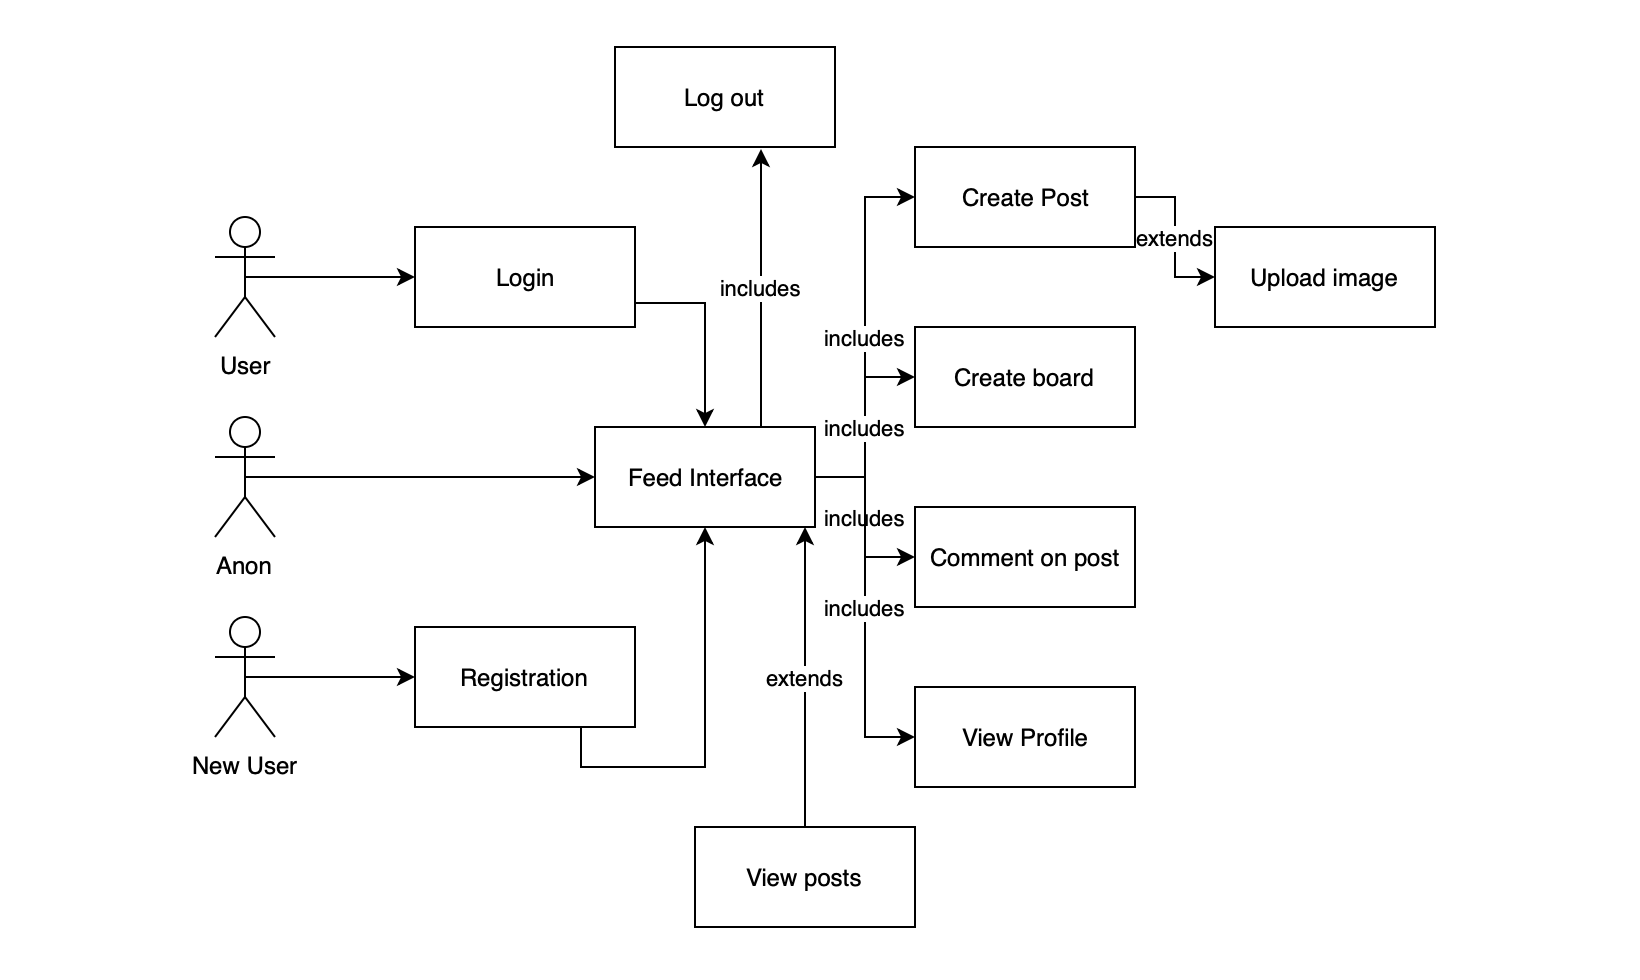
\includegraphics[width=0.91\textwidth]{diagram.png}
\caption{Interface Interaction Diagram}
\end{figure}

\subsection{Registration\index{registration}}
\begin{itemize}
    \item \textbf{ID} - FR1
    \item \textbf{Title} - User Registration
    \item \textbf{Brief description} - A new user have to register on the website to access the features if he/she wish to not try anonymous signin. User need to provide a email address and a password to register successfully.
    \item \textbf{Rational} - In order for user to register on website
    \item \textbf{Dependency} - None
\end{itemize}
\begin{figure}[h]
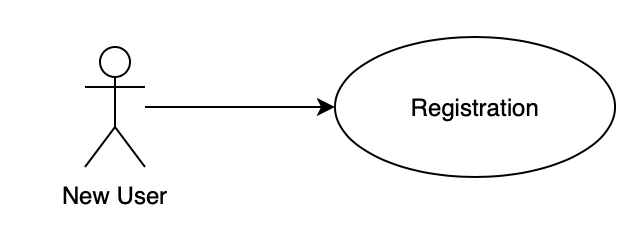
\includegraphics[width=0.5\textwidth]{registration.png}
\end{figure}

\subsection{Login\index{login}}
\begin{itemize}
    \item \textbf{ID} - FR2
    \item \textbf{Title} - User Login
    \item \textbf{Brief description} - Given that a user has registered, then the user should be able to log in to the website.
    \item \textbf{Rational} - In order for user to login
    \item \textbf{Dependency} - FR1
\end{itemize}
\begin{figure}[h]
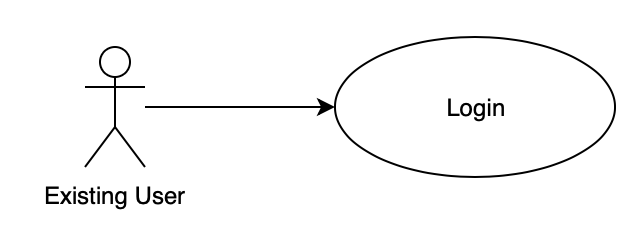
\includegraphics[width=0.5\textwidth]{login.png}
\end{figure}

\subsection{Feed Interface\index{feed interface}}
\begin{itemize}
    \item \textbf{ID} - FR3
    \item \textbf{Title} - Website's feed interface
    \item \textbf{Brief description} - This page will have different options such as to view profile, create post, comment, etc.
    \item \textbf{Rational} - In order to display various options that user can perform in this website.
    \item \textbf{Dependency} - FR2
\end{itemize}
\begin{figure}[h]
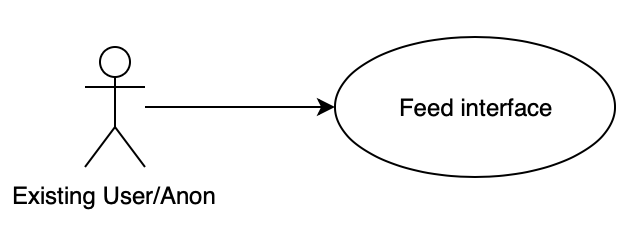
\includegraphics[width=0.5\textwidth]{feedinterface.png}
\end{figure}

\subsection{View Posts\index{view posts}}
\begin{itemize}
    \item \textbf{ID} - FR4
    \item \textbf{Title} - To view all posts
    \item \textbf{Brief description} - Here users will be able to view all the posts created by other users sorted in descending order.
    \item \textbf{Rational} - In order to display feeds to users
    \item \textbf{Dependency} - FR2, FR3
\end{itemize}
\begin{figure}[h]
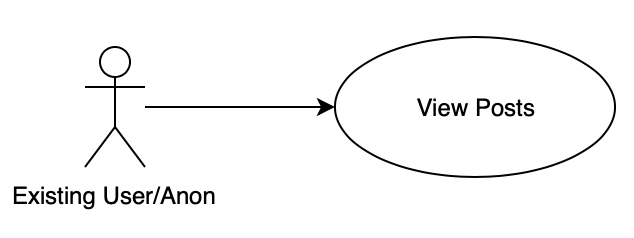
\includegraphics[width=0.5\textwidth]{viewpost.png}
\end{figure}

\subsection{Create Post\index{create post}}
\begin{itemize}
    \item \textbf{ID} - FR5
    \item \textbf{Title} - Creating a post
    \item \textbf{Brief description} - Users/Anon will be able to create post under a board.
    \item \textbf{Rational} - In order to create post
    \item \textbf{Dependency} - FR3
\end{itemize}
\begin{figure}[h]
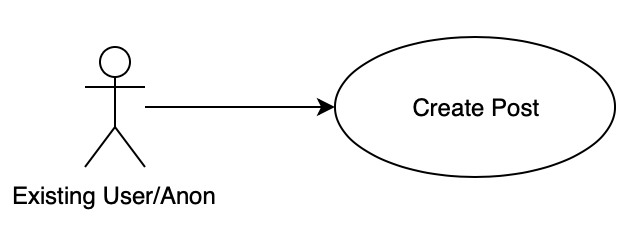
\includegraphics[width=0.5\textwidth]{createpost.png}
\end{figure}

\subsection{Upload Image\index{upload image}}
\begin{itemize}
    \item \textbf{ID} - FR6
    \item \textbf{Title} - Uploading an image for create post
    \item \textbf{Brief description} - In order to create a post users will need to upload images relevant to board.
    \item \textbf{Rational} - In order to create post with image
    \item \textbf{Dependency} - FR5
\end{itemize}
\begin{figure}[h]
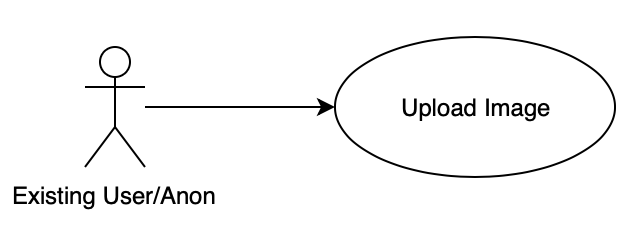
\includegraphics[width=0.5\textwidth]{uploadimage.png}
\end{figure}

\subsection{Create Board\index{create board}}
\begin{itemize}
    \item \textbf{ID} - FR7
    \item \textbf{Title} - Creating new sub-topic or board
    \item \textbf{Brief description} - If there is no existing topic of discussion then user can create a new subtopic for discussion i.e. a board.
    \item \textbf{Rational} - In order to create a new board
    \item \textbf{Dependency} - FR3
\end{itemize}
\begin{figure}[h]
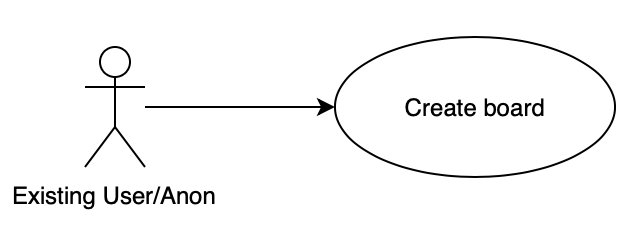
\includegraphics[width=0.5\textwidth]{createboard.png}
\end{figure}

\subsection{Comment on Post\index{comment}}
\begin{itemize}
    \item \textbf{ID} - FR8
    \item \textbf{Title} - Commenting on posts
    \item \textbf{Brief description} - For users to comment of the existing posts to share views about them.
    \item \textbf{Rational} - In order to comment on the post
    \item \textbf{Dependency} - FR4
\end{itemize}
\begin{figure}[h]
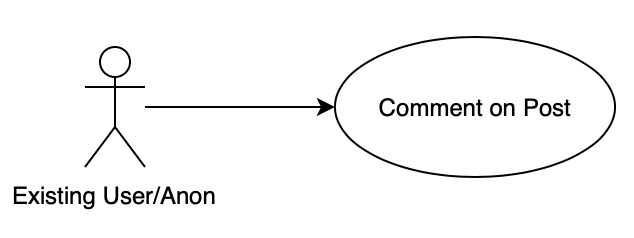
\includegraphics[width=0.5\textwidth]{comment.png}
\end{figure}

\subsection{View Profile\index{view profile}}
\begin{itemize}
    \item \textbf{ID} - FR9
    \item \textbf{Title} - To view user profile
    \item \textbf{Brief description} - Displays user details such as created posts and comments posted
    \item \textbf{Rational} - To view the user's profile for tracking
    \item \textbf{Dependency} - FR3
\end{itemize}
\begin{figure}[h]
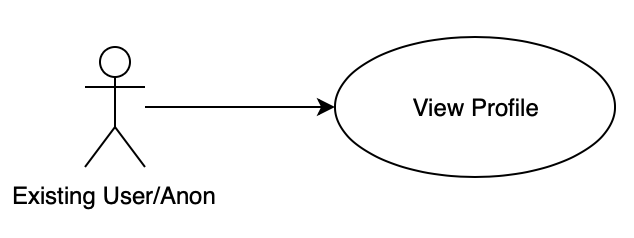
\includegraphics[width=0.5\textwidth]{viewprofile.png}
\end{figure}

\subsection{Logout\index{logout}}
\begin{itemize}
    \item \textbf{ID} - FR10
    \item \textbf{Title} - Sign-off from website
    \item \textbf{Brief description} - To sign-out from the website once the work is done
    \item \textbf{Rational} - To sign-out from the website
    \item \textbf{Dependency} - FR3, FR2
\end{itemize}
\begin{figure}[h]
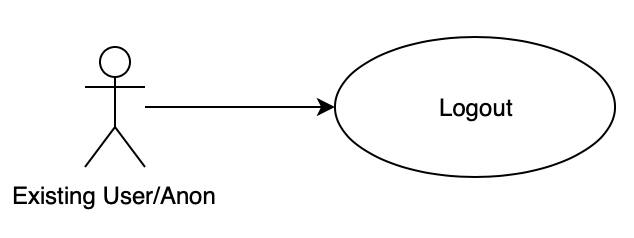
\includegraphics[width=0.5\textwidth]{logout.png}
\end{figure}
\vspace{2pt}

\section{User Interface requirements\index{user interface}}
This section covers the details of the required user interfaces 

\begin{figure}[H]
\centering
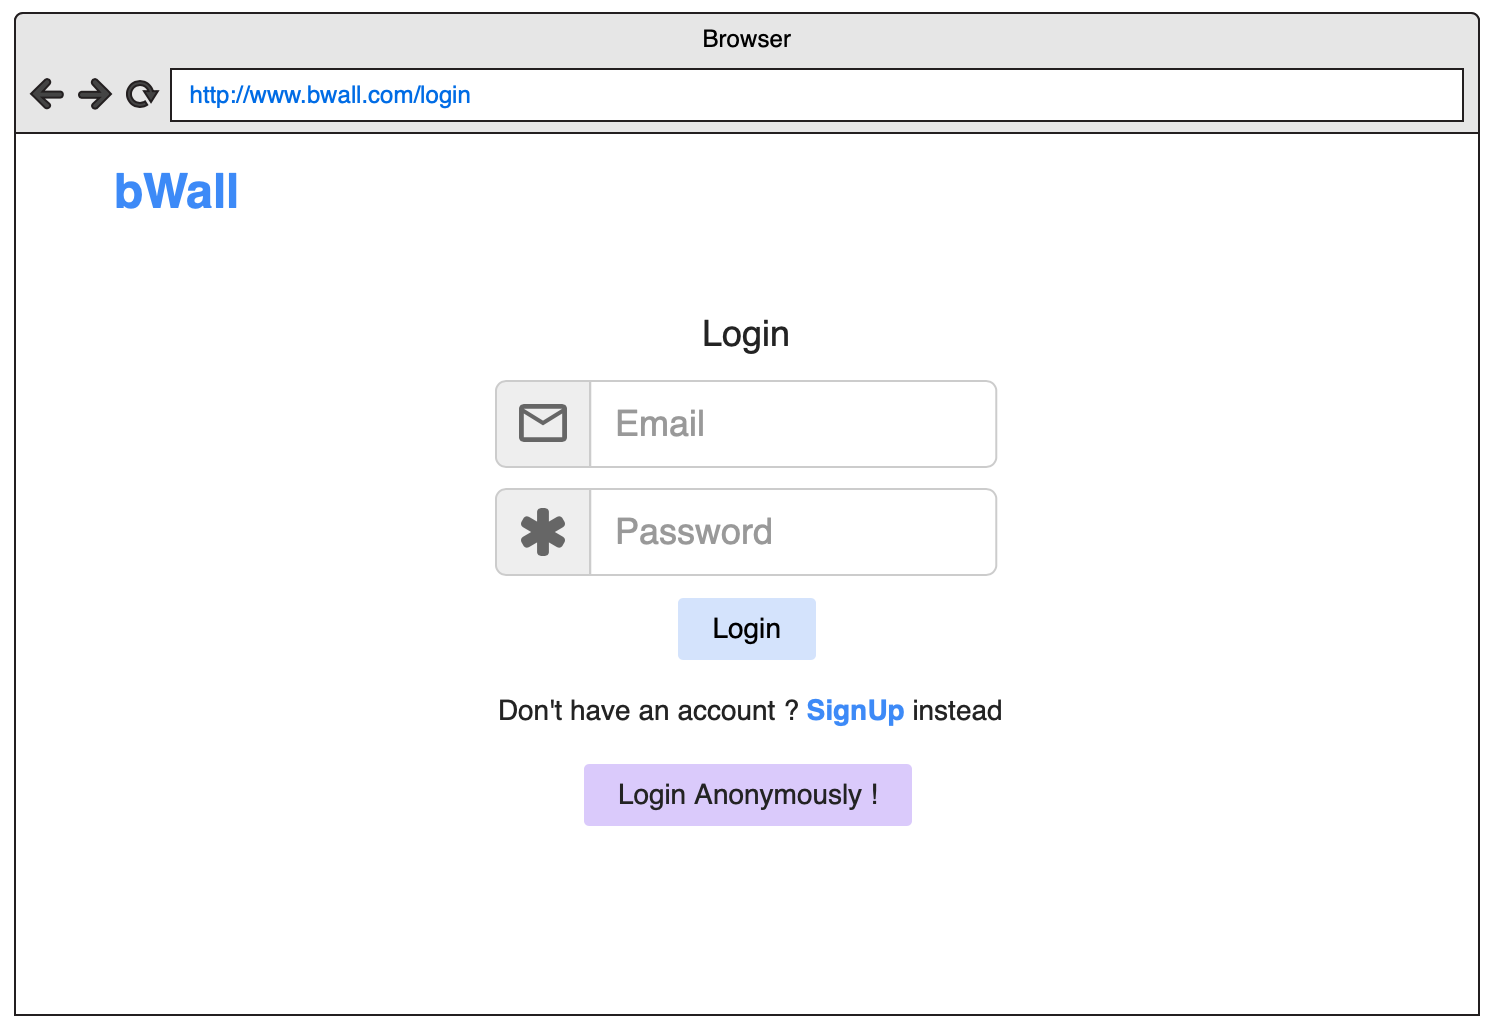
\includegraphics[width=12cm]{uilogin.png}
\caption{Login UI\index{login UI}}
\label{fig:loginui}
\end{figure}
This is the first component that the user will see when he/she will open the site. In the login UI (fig:\ref{fig:loginui}) user will be provided with two input fields of type email and password. User need to provide both and click on login button. If a user is new to the website they can also click on signup to register themselves or they can choose to browse anonymously.

Similarly the signup page (fig:\ref{fig:signupui}) contains two input fields of type email and password. After entering the details user can signup and the account will be created.

View Interface (fig:\ref{fig:viewinterfaceui}) holds all the details of current posts and different types of boards present in the website. This also is the first page after login and hold various options such as view profile, create board, etc.

\begin{figure}[H]
\centering
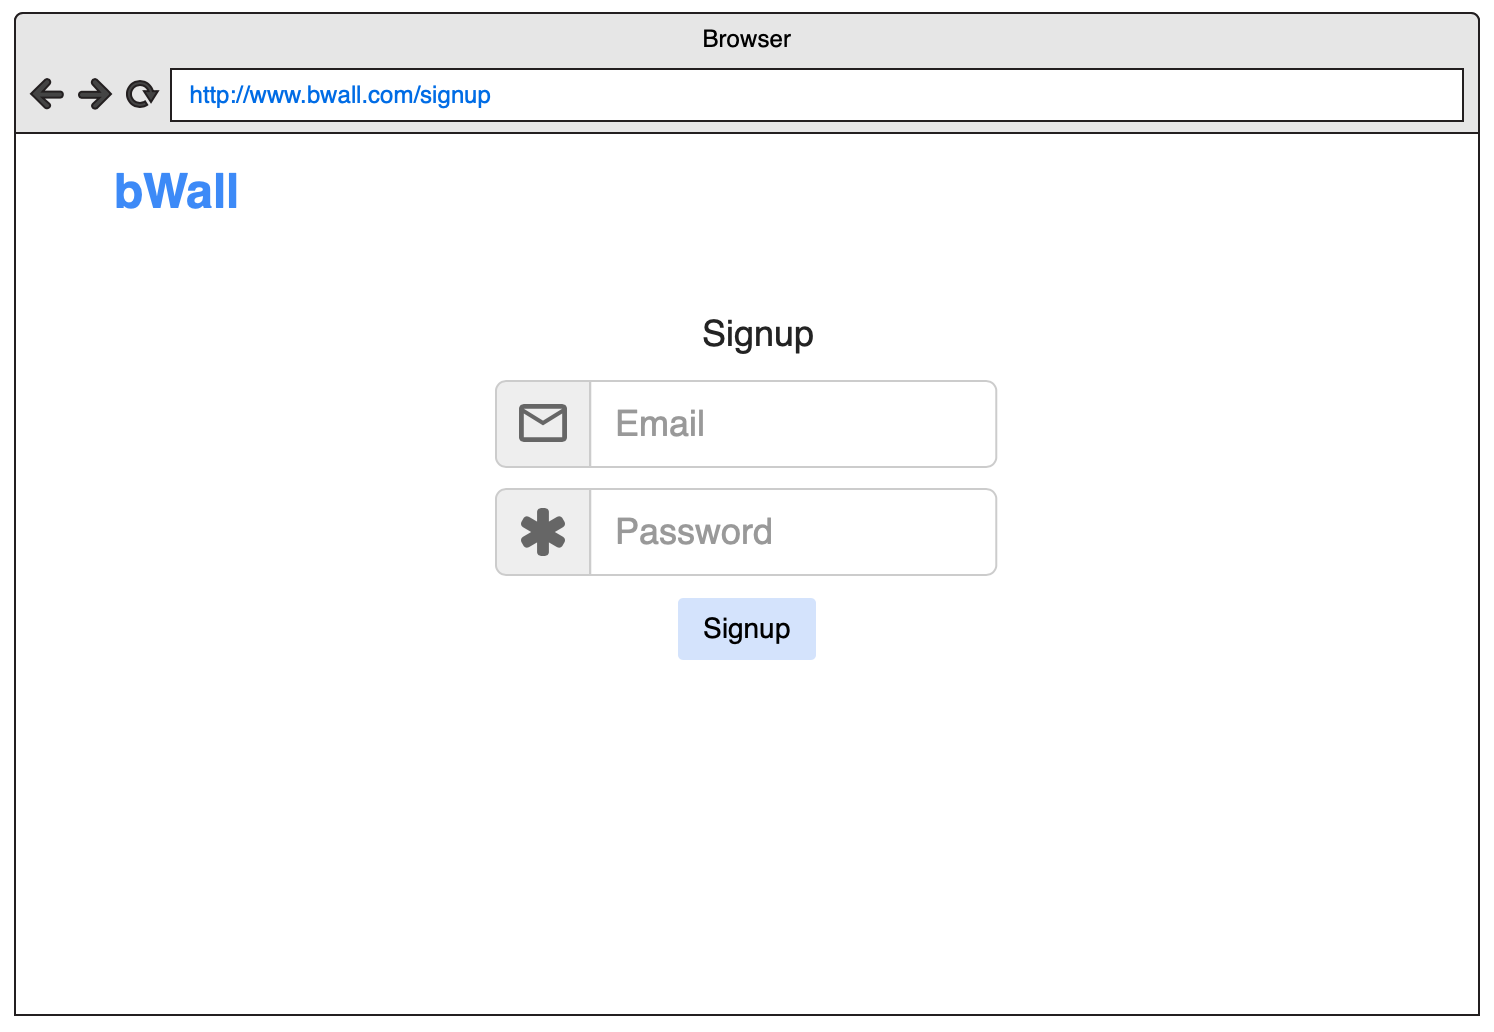
\includegraphics[width=12cm]{uisignup.png}
\caption{SignUp UI\index{signup UI}}
\label{fig:signupui}
\end{figure}
\begin{figure}[H]
\centering
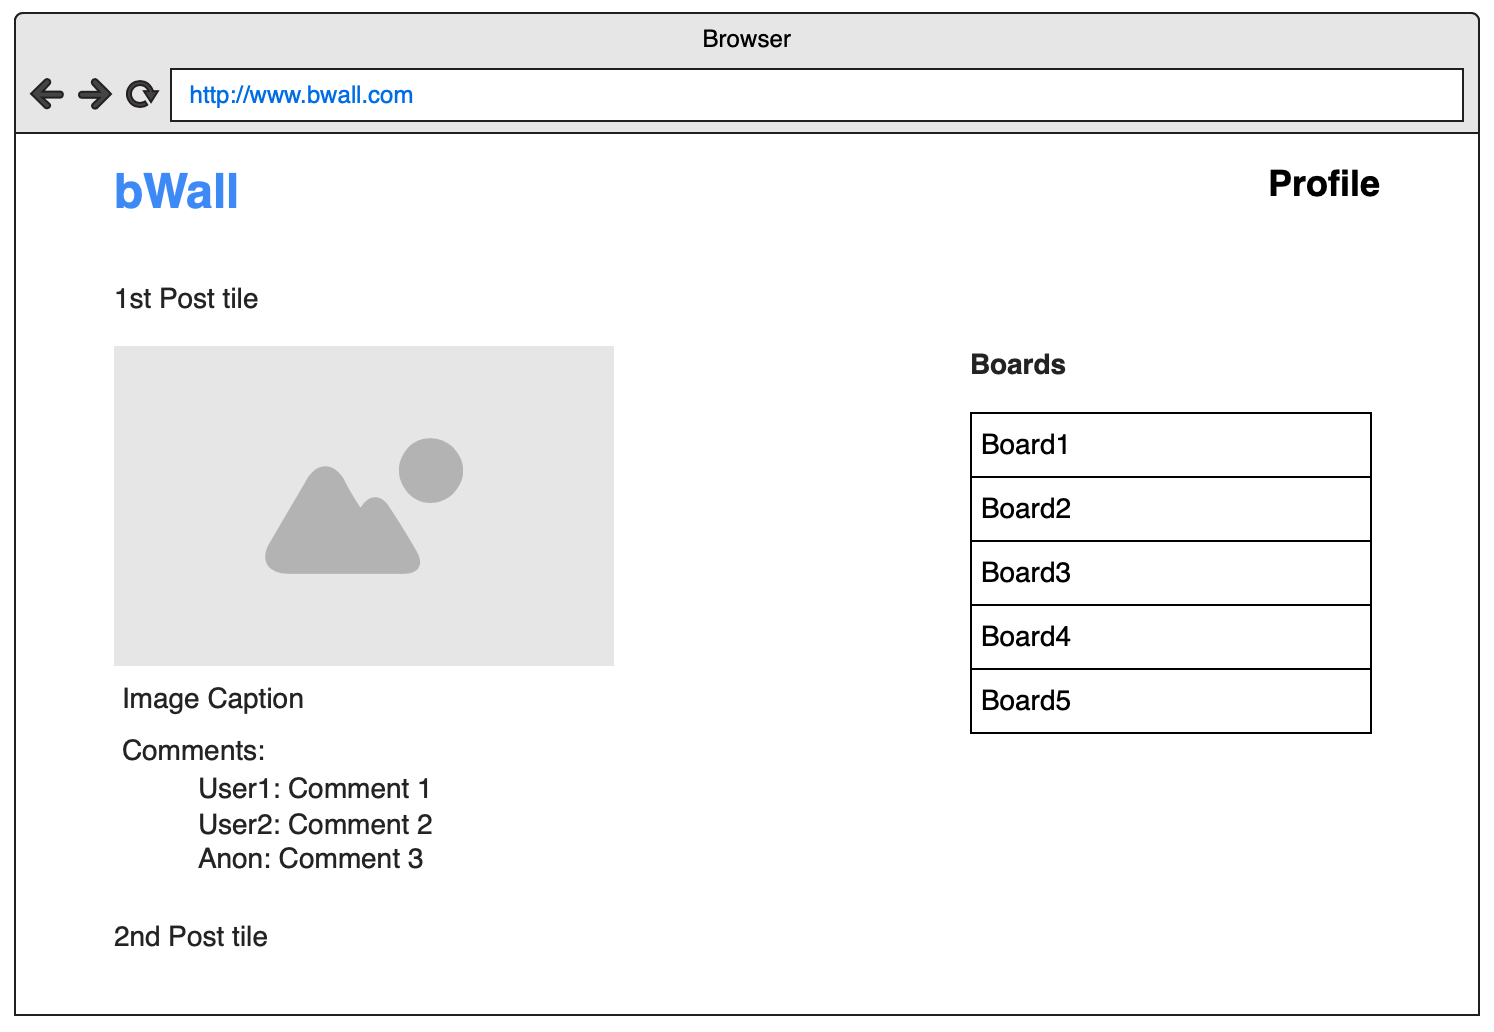
\includegraphics[width=12cm]{uiviewinterface.png}
\caption{View Interface\index{view interface UI}}
\label{fig:viewinterfaceui}
\end{figure}
\begin{figure}[H]
\centering
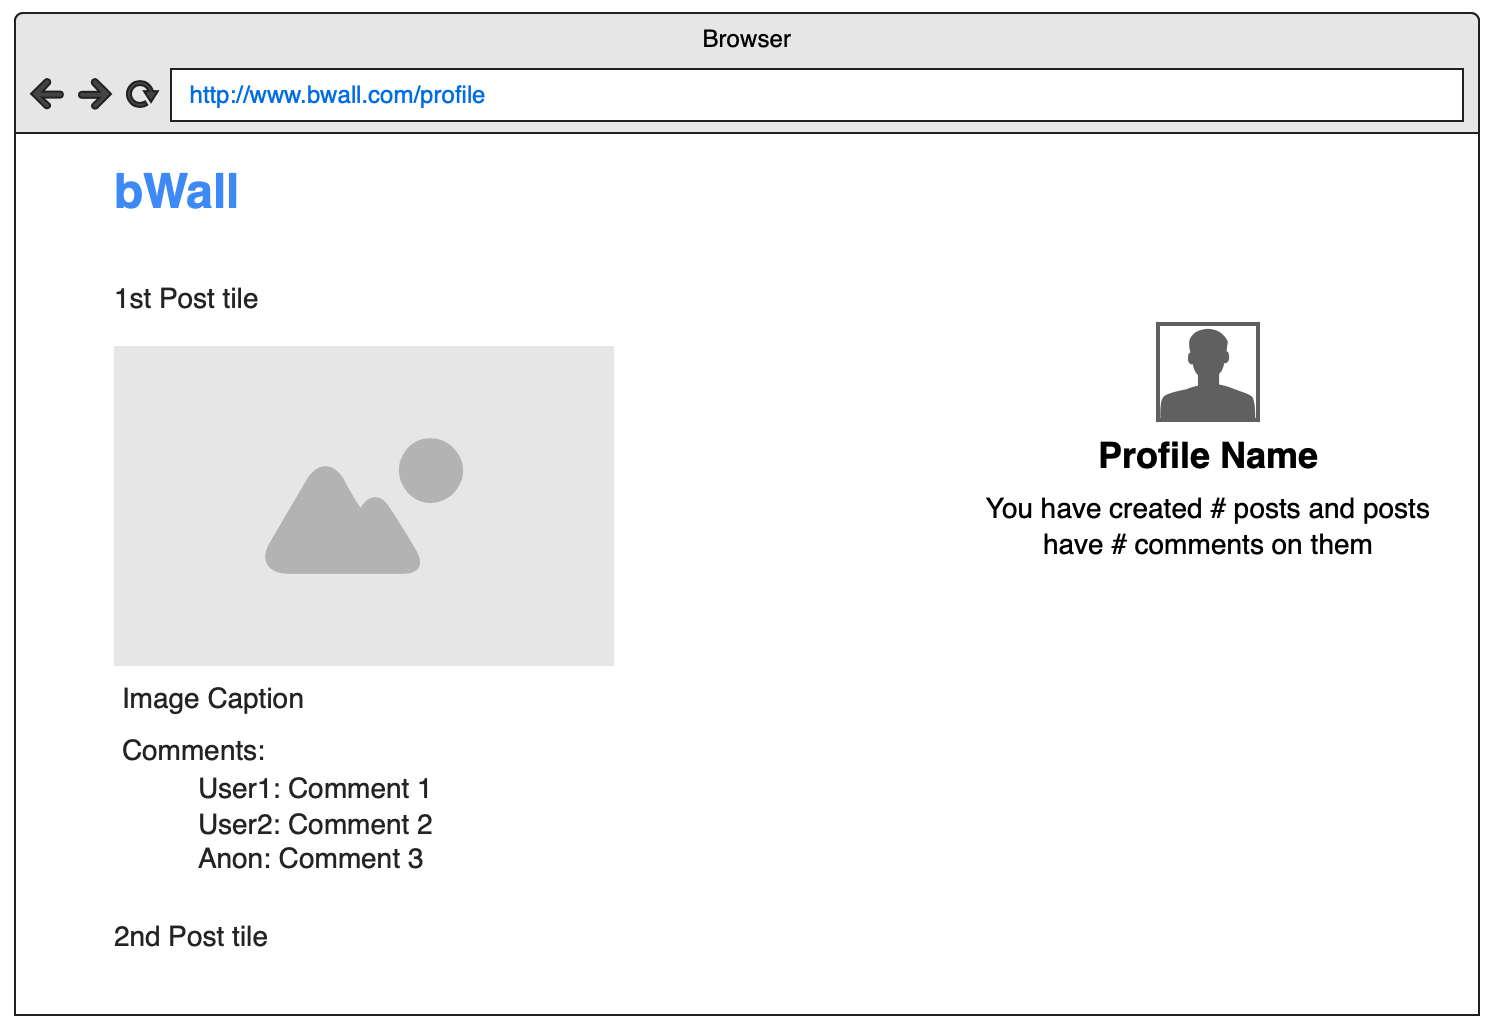
\includegraphics[width=12cm]{uiviewprofile.png}
\caption{Profile UI\index{profile UI}}
\label{fig:profileui}
\end{figure}
\begin{figure}[H]
\centering
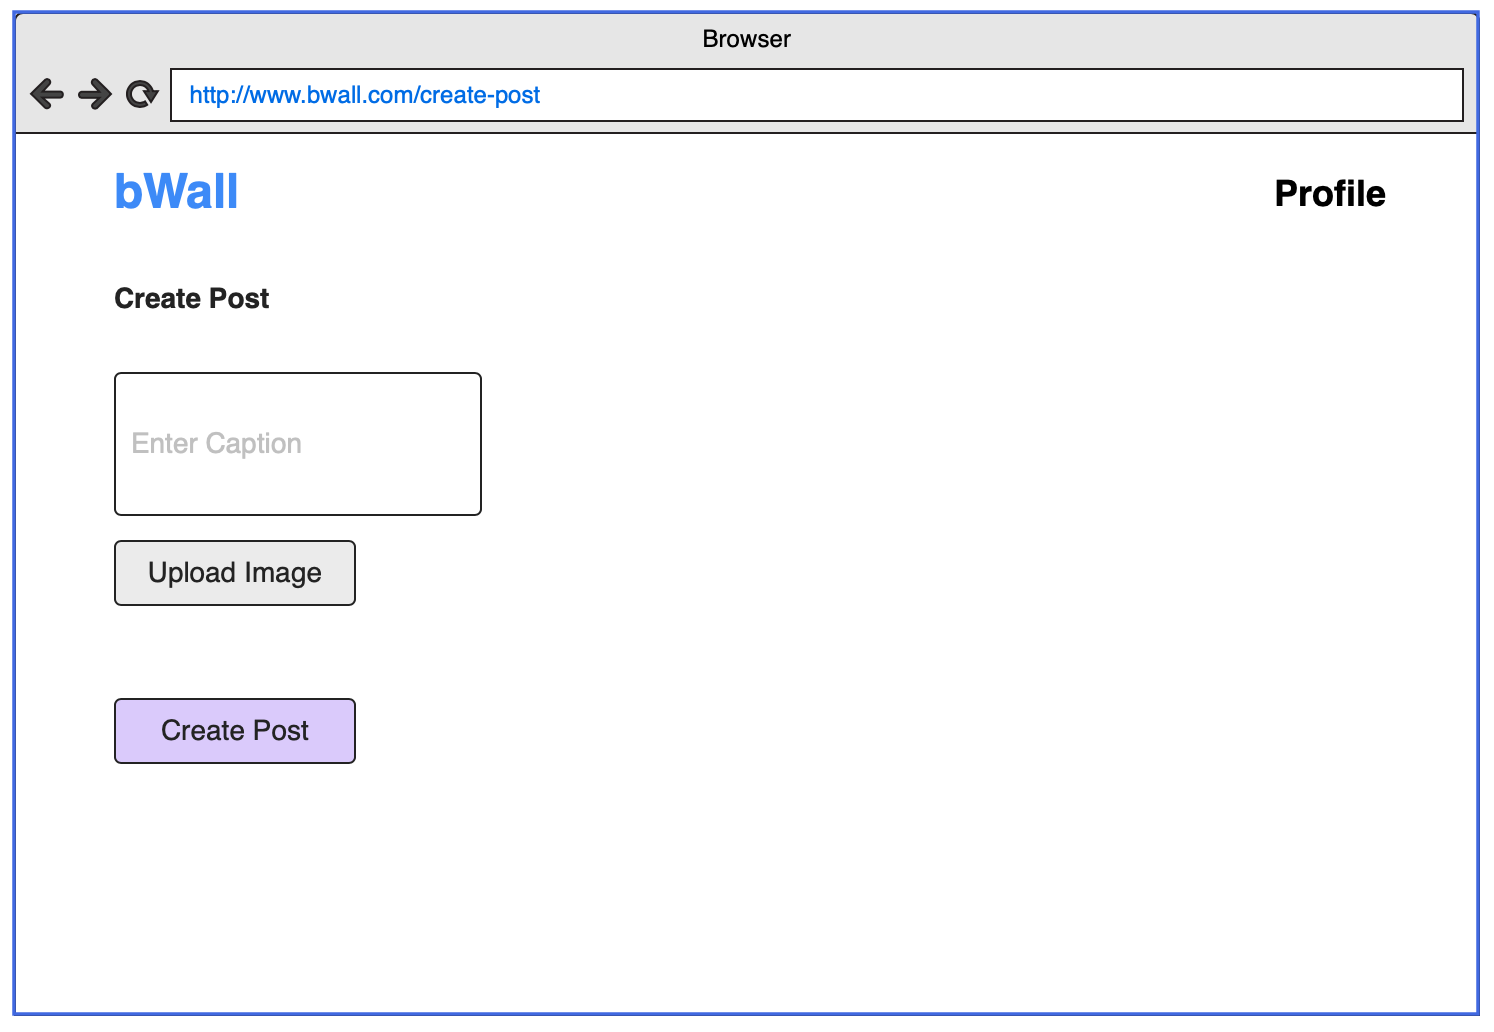
\includegraphics[width=12cm]{uicreatepost.png}
\caption{Create Post UI\index{create post UI}}
\label{fig:createpostui}
\end{figure}

The profile page (fig:\ref{fig:profileui}) contains the posts details created by the specific user. Its also shows the count of number of posts the user has created and the number of comments user as posted.

\begin{figure}[H]
\centering
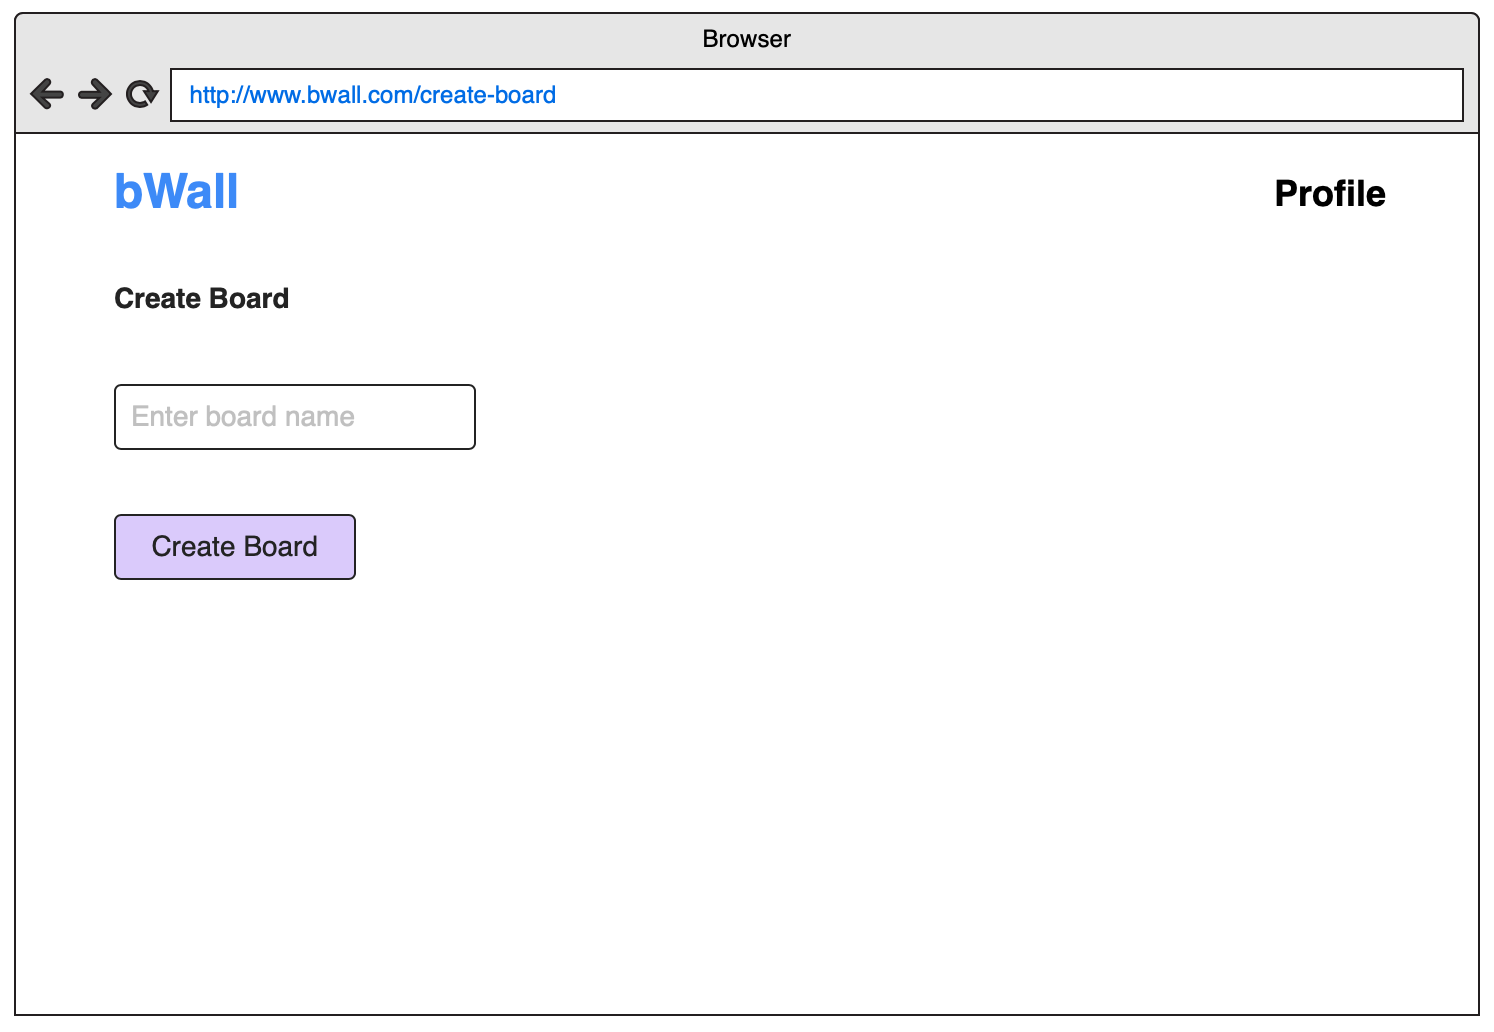
\includegraphics[width=12cm]{uicreateboard.png}
\caption{Create Board UI\index{create board UI}}
\label{fig:createboardui}
\end{figure}

Create post page (fig:\ref{fig:createpostui}) will allow user to create posts. Here user will be provided with the input field to enter the feed text and an option to upload the image.

Create board page (fig:\ref{fig:createboardui}) works in the similar fashion to that of create post page but only difference being that a new board will be created.

There can also be other UI elements to the website but only high-level UI elements are discussed here. There will also be other UI elements such as 404 page, logout page, terms and conditions page, etc.

\section{Performance requirements\index{performance requirements}}
The requirements in this section provide a detailed specification of the user interaction with the software and measurements placed on the system performance\index{system performance}.

\subsection{Posts viewing feature\index{post viewing}}

\begin{tabularx}{\textwidth} { 
  | >{\raggedright\arraybackslash}X 
  | >{\raggedright\arraybackslash}X |}
 \hline
 \textbf{ID} & QR1 \\
 \hline
 \textbf{Title}  & View Post features  \\
 \hline
 \textbf{Description} & Users must be able to see the posts flawlessly with very little time gap. \\
 \hline 
 \textbf{Dependency} & None \\
 \hline 
\end{tabularx}

\subsection{Create board and Create post usage}

\begin{tabularx}{\textwidth} { 
  | >{\raggedright\arraybackslash}X 
  | >{\raggedright\arraybackslash}X |}
 \hline
 \textbf{ID} & QR2 \\
 \hline
 \textbf{Title}  & Create board and Create post usage  \\
 \hline
 \textbf{Description} & User must be able to create post/board in quick manner with a very simple UI design. There operations must be done in a single click. \\
 \hline 
 \textbf{Dependency} & None \\
 \hline 
\end{tabularx}

\subsection{Response Time\index{response time}}

\begin{tabularx}{\textwidth} { 
  | >{\raggedright\arraybackslash}X 
  | >{\raggedright\arraybackslash}X |}
 \hline
 \textbf{ID} & QR3 \\
 \hline
 \textbf{Title}  & Response Time  \\
 \hline
 \textbf{Description} & The fastness of the post creation or display. It should take no more than 2 seconds 100\% of the time. \\
 \hline 
 \textbf{Dependency} & None \\
 \hline 
\end{tabularx}

\subsection{System Dependability\index{system dependability}}

\begin{tabularx}{\textwidth} { 
  | >{\raggedright\arraybackslash}X 
  | >{\raggedright\arraybackslash}X |}
 \hline
 \textbf{ID} & QR4 \\
 \hline
 \textbf{Title}  & System dependability  \\
 \hline
 \textbf{Description} & If the system loses the connection to the Internet or the system gets some strange input, the user should be informed. The user will be directed to a custom 404 page. \\
 \hline 
 \textbf{Dependency} & None \\
 \hline 
\end{tabularx}

\section{Non-Functional Requirements\index{non-functional requirements}}
This section discusses the five non-functional requirements mainly security, reliability, maintainability, scalability, and usability.

\subsection{Security\index{security}}
The website will be hosted on a third party server provider such as Amazon AWS\index{AWS} which is very secure as it is monitored by Amazon Security. The user details such as email-id and password will be first hashed and then encrypted\index{encrypted} and then stored into the database table such that there is no risk of direct attack to the database\index{database}. The website will be secured from SQL attacks using inbuilt backend framework security module.

\subsection{Reliability\index{reliability}}
In case of any failure to the site services the user will be informed about the issue. There will be exception handling involved for each function discussed above. If there is an issue the team will ensure that the user must not face a downtime\index{downtime} of more than 30 minutes. Also special care is taken via server providers that the downtime issue is faced by the user only at most once in a year.

\subsection{Maintainability\index{maintainability}}
Our team is dedicated to write clean code using OOPs concepts and comments where necessary. Any other person can easily adapt to the coding style of the website. Apart from code, the maintainability costs in terms of hosting\index{hosting} depends upon the user scale. If the number of users increase then the cost can go up. As the product hit larger requests the site will tend to crash and will require faster servers to maintain the flow. 

\subsection{Scalability\index{scalability}}
As long as the user base is limited to a small number ~1000 users there is no need to worry about scalability. But is the user base increase then the website needs to be scaled horizontally using microservice\index{microservice} architecture. The backend system used in the website building already provides a solution for scaling the website hence it can be done easily at need-per-basis.

\subsection{Usability}
The product is designed in such a way that each type of customer will be able to use it at ease. The learning curve for a standard user using internet for at least a year is pretty easy. Users will have a pleasant viewing experience and each section of the product will provide a description information of what that section does. 


\printindex





\end{document}
